\documentclass[11pt]{article}

\usepackage[margin=1in]{geometry}
\usepackage{graphicx}
\usepackage{booktabs}
\usepackage{amsmath}
\usepackage{hyperref}
\usepackage{xcolor}
\usepackage{caption}

\definecolor{darkgreen}{RGB}{0,120,0}
\definecolor{darkred}{RGB}{180,0,0}
\newcommand{\worked}[1]{\textcolor{darkgreen}{\textbf{#1}}}
\newcommand{\failed}[1]{\textcolor{darkred}{\textbf{#1}}}

\title{Uncertainty Signal Pilot: Perception and Reasoning Entropy\\
\large FERMAT Handwritten Math, Qwen2.5-VL-3B}
\author{}
\date{\today}

\begin{document}
\maketitle

\begin{abstract}
This pilot tests whether two entropy-based uncertainty signals -- \emph{perception
entropy} (instability in transcribing a handwritten math answer) and
\emph{reasoning entropy} (instability in grading whether an answer contains an
error) -- carry real signal about model correctness, on 100 items from the
FERMAT dataset with Qwen2.5-VL-3B. Perception entropy required two failed
approaches before a working one was found; the final version achieves
AUROC~$=0.79$ with clearly visible separation between correct and incorrect
items. Reasoning entropy's digit-only pipeline was clean from the start but the
signal is weak (AUROC~$=0.62$ at $K=5$); resampling to $K=15$ confirmed the
signal is real (the exact tie between correct/incorrect medians at $K=5$
breaks) but only modestly stronger (AUROC~$=0.665$). A follow-up experiment
clustering the model's own \verb|**Reasoning:**| explanation text -- rather than
only its parsed \verb|**Error:**| digit -- found a substantially stronger signal
(AUROC~$=0.702$ at $K=5$, without any additional sampling), traced to a
concrete cause: in 12\% of samples the model's final digit contradicts its own
just-written reasoning, and the digit is the noisier of the two.
\end{abstract}

\section{Goal}

Given a vision-language model transcribing and grading handwritten math answers,
does the entropy of its own repeated outputs -- how much it disagrees with
itself across independent samples -- predict when it is actually wrong? This is
a fast, scoped-down pilot to check whether either signal exists at all, not the
full study: no bootstrap confidence intervals, no baseline suite, no conformal
calibration, no human double grading, no full-dataset run.

\section{Setup}

\begin{itemize}
  \item \textbf{Data}: 100 items sampled (seed 42) from the FERMAT dataset.
  \item \textbf{Model}: Qwen2.5-VL-3B-Instruct.
  \item \textbf{Perception}: the model transcribes a handwritten Question--Answer
    pair; $K=5$ samples at temperature 0.7, plus 2 samples at temperature 0 as a
    determinism sanity anchor.
  \item \textbf{Reasoning}: the model grades whether the handwritten Answer
    contains an error (binary 0/1); same $K=5$ + 2 temperature-0 sampling scheme.
  \item \textbf{Entropy}: Shannon entropy in nats over the cluster distribution
    of the $K$ sampled outputs for one item, $H = -\sum_i p_i \ln p_i$.
  \item \textbf{Correctness labels}: transcription is compared against the
    ground-truth answer; grading is compared against the ground-truth
    error label.
\end{itemize}

\section{Perception Entropy: Two Failures, One Fix}

\subsection{Attempt 1: exact-string clustering \failed{(failed)}}

The transcription prompt asks for the \emph{full} handwritten derivation, not
just a final answer. Clustering by exact string match after light
normalization treated any paraphrasing of that derivation as a different
answer.

\begin{center}
\begin{tabular}{lc}
\toprule
Items pinned at maximum entropy ($\ln 5 \approx 1.609$) & 83/100 \\
\bottomrule
\end{tabular}
\end{center}

83\% of items showed the maximum possible disagreement regardless of whether
the model actually agreed with itself on the substance of the answer --
the metric carried essentially no information.

\subsection{Attempt 2: naive semantic clustering \failed{(failed)}}

Reasoning that exact-match was too strict, the next attempt clustered by
semantic similarity instead: bidirectional NLI entailment and, separately,
embedding cosine similarity, both applied to the whole derivation.

\begin{center}
\begin{tabular}{lccc}
\toprule
 & Canonical (Attempt 1) & NLI & Embedding \\
\midrule
Mean entropy & 1.535 & 0.137 & 0.185 \\
Items at max entropy & 83/100 & 0/100 & 0/100 \\
\bottomrule
\end{tabular}
\end{center}

This looked like a fix -- entropy dropped sharply -- but the correctness rate
that came with it (majority-vote transcription matched against ground truth
via the same NLI entailment check) was $92/97 = 95\%$, implausibly high next
to the model's other performance figures. Inspection showed the cause: with
premise and hypothesis sharing nearly identical scaffolding (the same LaTeX
structure, the same boilerplate phrasing), the NLI model's well-documented
lexical-overlap bias pushed it toward ``entailment'' regardless of whether a
buried number or coefficient actually differed. The fix for Attempt~1's
problem introduced a new, opposite failure mode: over-merging.

\subsection{Attempt 3: final-answer extraction \worked{(worked)}}

The actual defect in both prior attempts was comparing the \emph{wrong span of
text}: the full derivation, when only the final answer matters for a
correctness judgment. Attempt 3 extracts just the final answer -- the last
multiple-choice option statement, a \verb|\boxed{}| result, the last
display-math block, or (rarest) the last line -- before clustering with the
same syntactic/canonicalization approach as Attempt~1.

\begin{center}
\begin{tabular}{lc}
\toprule
Metric & Value \\
\midrule
AUROC (perception entropy $\rightarrow$ transcription error) & \textbf{0.788} \\
Items at max entropy & 14/100 \\
Transcription correct & 42/100 \\
Median entropy, correct group ($n=42$) & 0.500 \\
Median entropy, incorrect group ($n=58$) & 1.332 \\
Mean entropy, correct group & 0.583 \\
Mean entropy, incorrect group & 1.099 \\
\bottomrule
\end{tabular}
\end{center}

This is the strongest result in the pilot: real, visible separation between
correct and incorrect items (Figure~\ref{fig:both-arms}, left panel).

\section{Reasoning Entropy: Clean Pipeline, Weak but Real Signal}

Unlike perception, the reasoning/grading pipeline required no comparable fix.
It clusters a single parsed binary digit (error present/absent) rather than
free text, so it never had the ``wrong span'' problem. The pipeline was
independently re-verified by recomputing correctness from scratch for all 100
items against the stored results: zero mismatches.

\subsection{$K=5$ baseline}

\begin{center}
\begin{tabular}{lc}
\toprule
Metric & Value \\
\midrule
AUROC (reasoning entropy $\rightarrow$ grading error) & 0.618 \\
Grading accuracy & 75\% \\
Median entropy, correct group ($n=75$) & 0.5004 \\
Median entropy, incorrect group ($n=25$) & 0.5004 \\
\bottomrule
\end{tabular}
\end{center}

The medians are \emph{exactly} tied. With only 5 samples of a binary outcome,
there are just 3 realistic entropy values (unanimous, a 4--1 split, a 3--2
split), which structurally limits how well two groups can be told apart by
this statistic.

\subsection{$K=15$ follow-up: is the weak signal a real ceiling, or under-sampling?}

To test whether $K=5$ was simply too coarse to reveal a real effect, grading
was resampled to $K=15$ for the same 100 items (reusing the original 5
samples and drawing 10 more), keeping perception untouched.

\begin{center}
\begin{tabular}{lcc}
\toprule
Metric & $K=5$ & $K=15$ \\
\midrule
AUROC & 0.618 & 0.665 \\
Grading accuracy & 75\% & 82\% \\
Distinct entropy values reached & 5 & 13 \\
Median entropy, correct group & 0.500 & 0.439 \\
Median entropy, incorrect group & 0.500 & 0.608 \\
\bottomrule
\end{tabular}
\end{center}

The exact median tie \emph{does} break at $K=15$ (Figure~\ref{fig:k-comparison}) --
real evidence that $K=5$ was not measuring nothing. But the improvement is
modest, not dramatic: a pre-registered decision rule (AUROC $\geq 0.72$
\emph{and} the median tie breaking, to count as ``sharper''; $0.55$--$0.72$ as
``real but modest''; below $0.55$ as ``noise'') classifies this result as
\textbf{confirmed\_modest}. This pointed at a different question: is more
sampling the right lever at all, or is the \emph{digit itself} too coarse a
readout of the model's judgment?

\subsection{Reasoning-text clustering: a stronger, less noisy signal \worked{(worked)}}

The grading prompt asks the model to write a \verb|**Reasoning:**| explanation
before its \verb|**Error:**| digit. Every analysis so far discarded that
explanation and kept only the digit. Clustering the reasoning text instead --
via the same bidirectional NLI entailment approach that failed for perception
(Attempt 2) -- was tested against the already-collected $K=5$ raw samples, at
no additional GPU cost.

\begin{center}
\begin{tabular}{lcc}
\toprule
Metric & Digit-only & Reasoning-text \\
\midrule
AUROC & 0.618 & \textbf{0.702} \\
Median entropy, correct group ($n=75$) & 0.500 & 0.950 \\
Median entropy, incorrect group ($n=25$) & 0.500 (tied) & 1.332 \\
\bottomrule
\end{tabular}
\end{center}

Given that the same NLI approach caused Attempt 2's over-merging failure on
perception, this result was not trusted without directly checking for the same
bias. The check: do any two samples that \emph{disagree on the parsed digit}
(one says error, one says no error) ever get merged into the same
reasoning-text cluster? They do -- 55 times across the 61 items where samples
disagreed on the digit. Inspecting a diverse sample of these merges (8 cases,
different items) showed 7 of 8 were not opposed reasoning merged by mistake:
\emph{both} texts explicitly argued ``there is an error,'' just citing
different specific details, while their own digits disagreed. Quantified
across the full dataset: \textbf{60/494 samples (12\%)} have digit$=0$ while
their own reasoning opens by flagging a mistake (``incorrect,'' ``error,''
``mistake,'' ...). The model is self-contradicting within single samples --
writing a reasoning that argues for an error, then emitting the opposite digit
anyway, plausibly decoding noise on the final token, independent of the
fully-formed judgment already written. Reasoning-text clustering is not an
artifact of NLI bias; it is a readout that is not vulnerable to this specific
noise source the way the digit alone is (Figure~\ref{fig:reasoning-text}).

A GPU-accelerated confirmation of this result at $K=15$ (impractical on local
CPU -- $O(K^2)$ pairwise NLI comparisons make a full 100-item pass at $K=15$
take 1--2 hours locally) is in progress via a dedicated Colab notebook
(\texttt{pilot/02\_reasoning\_text\_entropy.ipynb}); results were not yet
available at the time of writing.

\section{Integrity Checks}

Both entropy signals depend on the sampling and parsing pipeline actually
working. Two checks validate that before trusting any entropy number.

\begin{center}
\begin{tabular}{lc}
\toprule
Check & Result \\
\midrule
Temperature-0 anchor, transcription (2 greedy draws/item, must be $\approx 0$) & 0/100 non-zero \\
Temperature-0 anchor, grading (2 greedy draws/item, must be $\approx 0$) & 0/100 non-zero \\
Transcription parse-failure rate (before marker-regex fix) & 13.4\% (67/500) \\
Transcription parse-failure rate (after marker-regex fix) & 4.0\% (20/500) \\
Grading parse-failure rate ($K=5$) & 1.0\% (5/500) \\
Grading parse-failure rate ($K=15$) & 0.9\% (14/1500) \\
\bottomrule
\end{tabular}
\end{center}

The temperature-0 anchor passing at 0/100 confirms the sampling/parsing
pipeline is behaving deterministically at temperature 0, as it must. The
transcription parse-failure rate was itself a real bug (the extraction regex
only matched the exact \verb|**Answer:**| markdown the prompt requested, missing
common real-world drift such as \LaTeX{} \verb|\textbf{}| bold, plain text, and
a full-width colon); widening the pattern recovered most of the missed samples.

\section{Summary}

\begin{center}
\begin{tabular}{lccc}
\toprule
Arm & Status & AUROC & Notes \\
\midrule
Perception (final) & \worked{Working} & 0.788 & Strong, visible separation \\
Perception (attempt 1) & \failed{Failed} & -- & 83\% pinned at max entropy \\
Perception (attempt 2) & \failed{Failed} & -- & Over-merged, 95\% implausible \\
Reasoning, digit-only ($K=5$) & \worked{Working} & 0.618 & Real but weak, medians tied \\
Reasoning, digit-only ($K=15$) & \worked{Working} & 0.665 & Confirmed modest, near ceiling \\
Reasoning, text-clustering ($K=5$) & \worked{Working} & \textbf{0.702} & Best reasoning-arm result; validated \\
Reasoning, text-clustering ($K=15$) & \emph{pending} & -- & GPU confirmation in progress \\
\bottomrule
\end{tabular}
\end{center}

\begin{figure}[htbp]
  \centering
  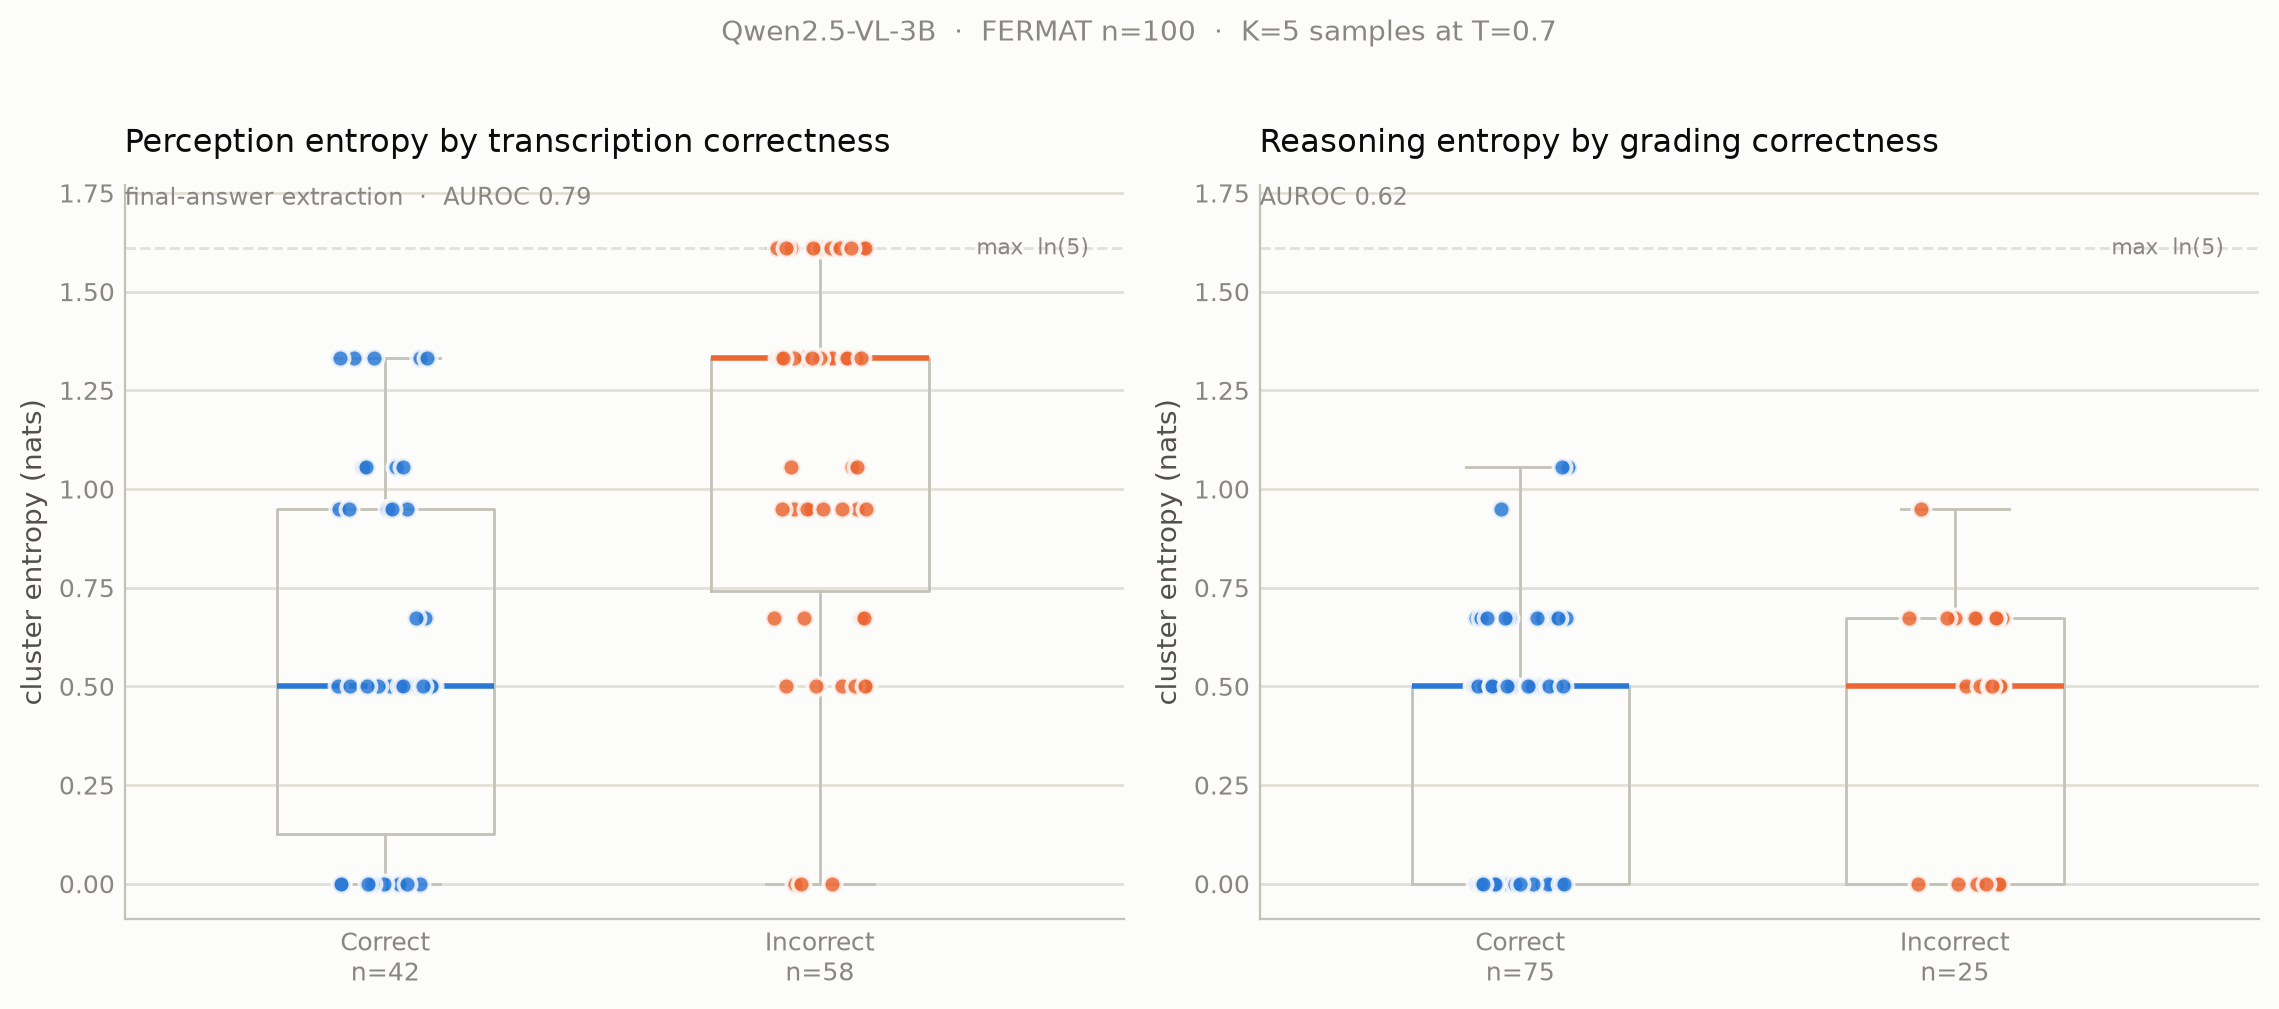
\includegraphics[width=\textwidth]{figures/final_both_arms_n100.png}
  \caption{Final result for both arms, $n=100$. Left: perception entropy by
  transcription correctness (AUROC 0.79). Right: reasoning entropy by grading
  correctness at $K=5$ (AUROC 0.62).}
  \label{fig:both-arms}
\end{figure}

\begin{figure}[htbp]
  \centering
  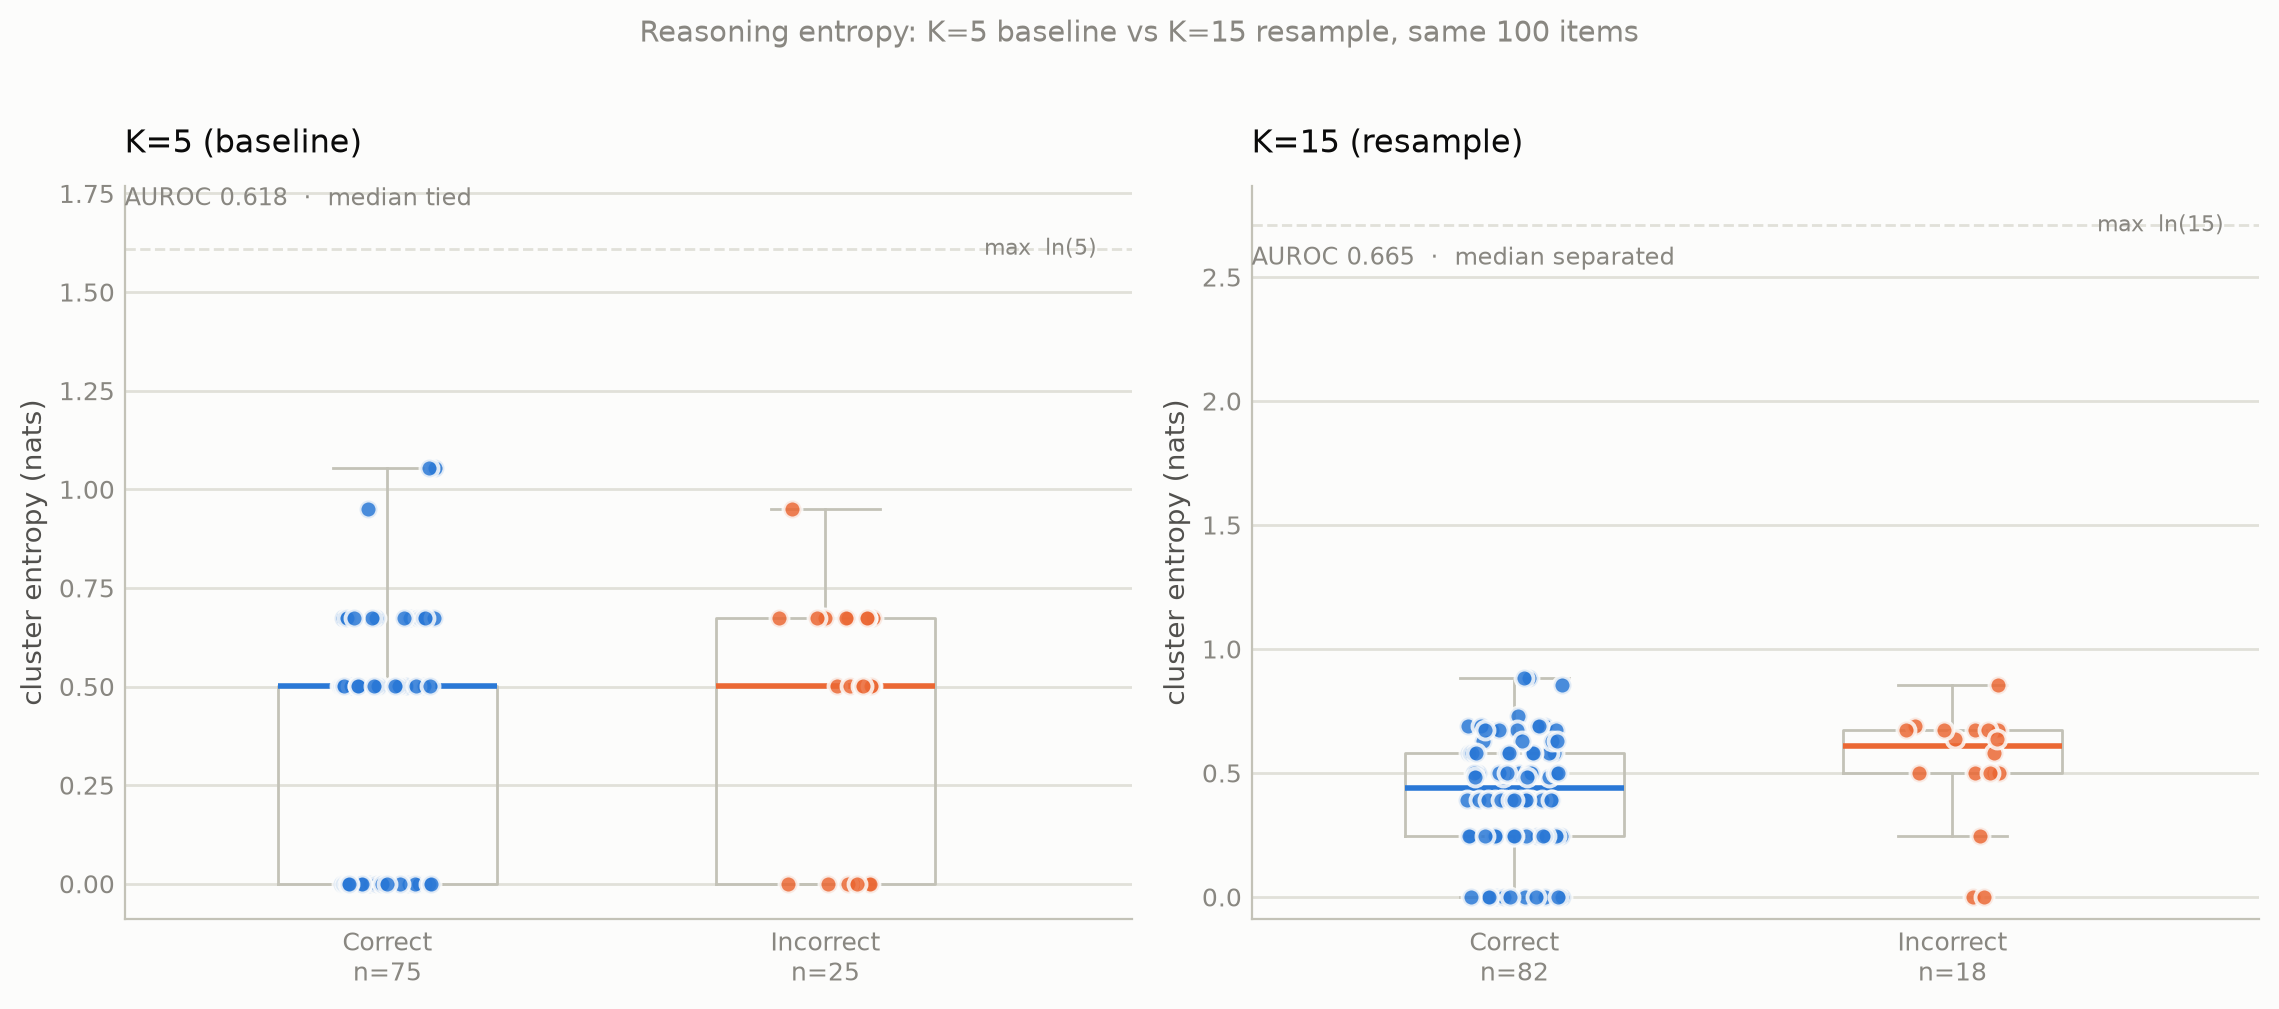
\includegraphics[width=\textwidth]{figures/k5_vs_k15_comparison.png}
  \caption{Reasoning entropy before ($K=5$) and after ($K=15$) resampling, same
  100 items. The exact median tie at $K=5$ breaks at $K=15$, but the overall
  separation remains modest.}
  \label{fig:k-comparison}
\end{figure}

\begin{figure}[htbp]
  \centering
  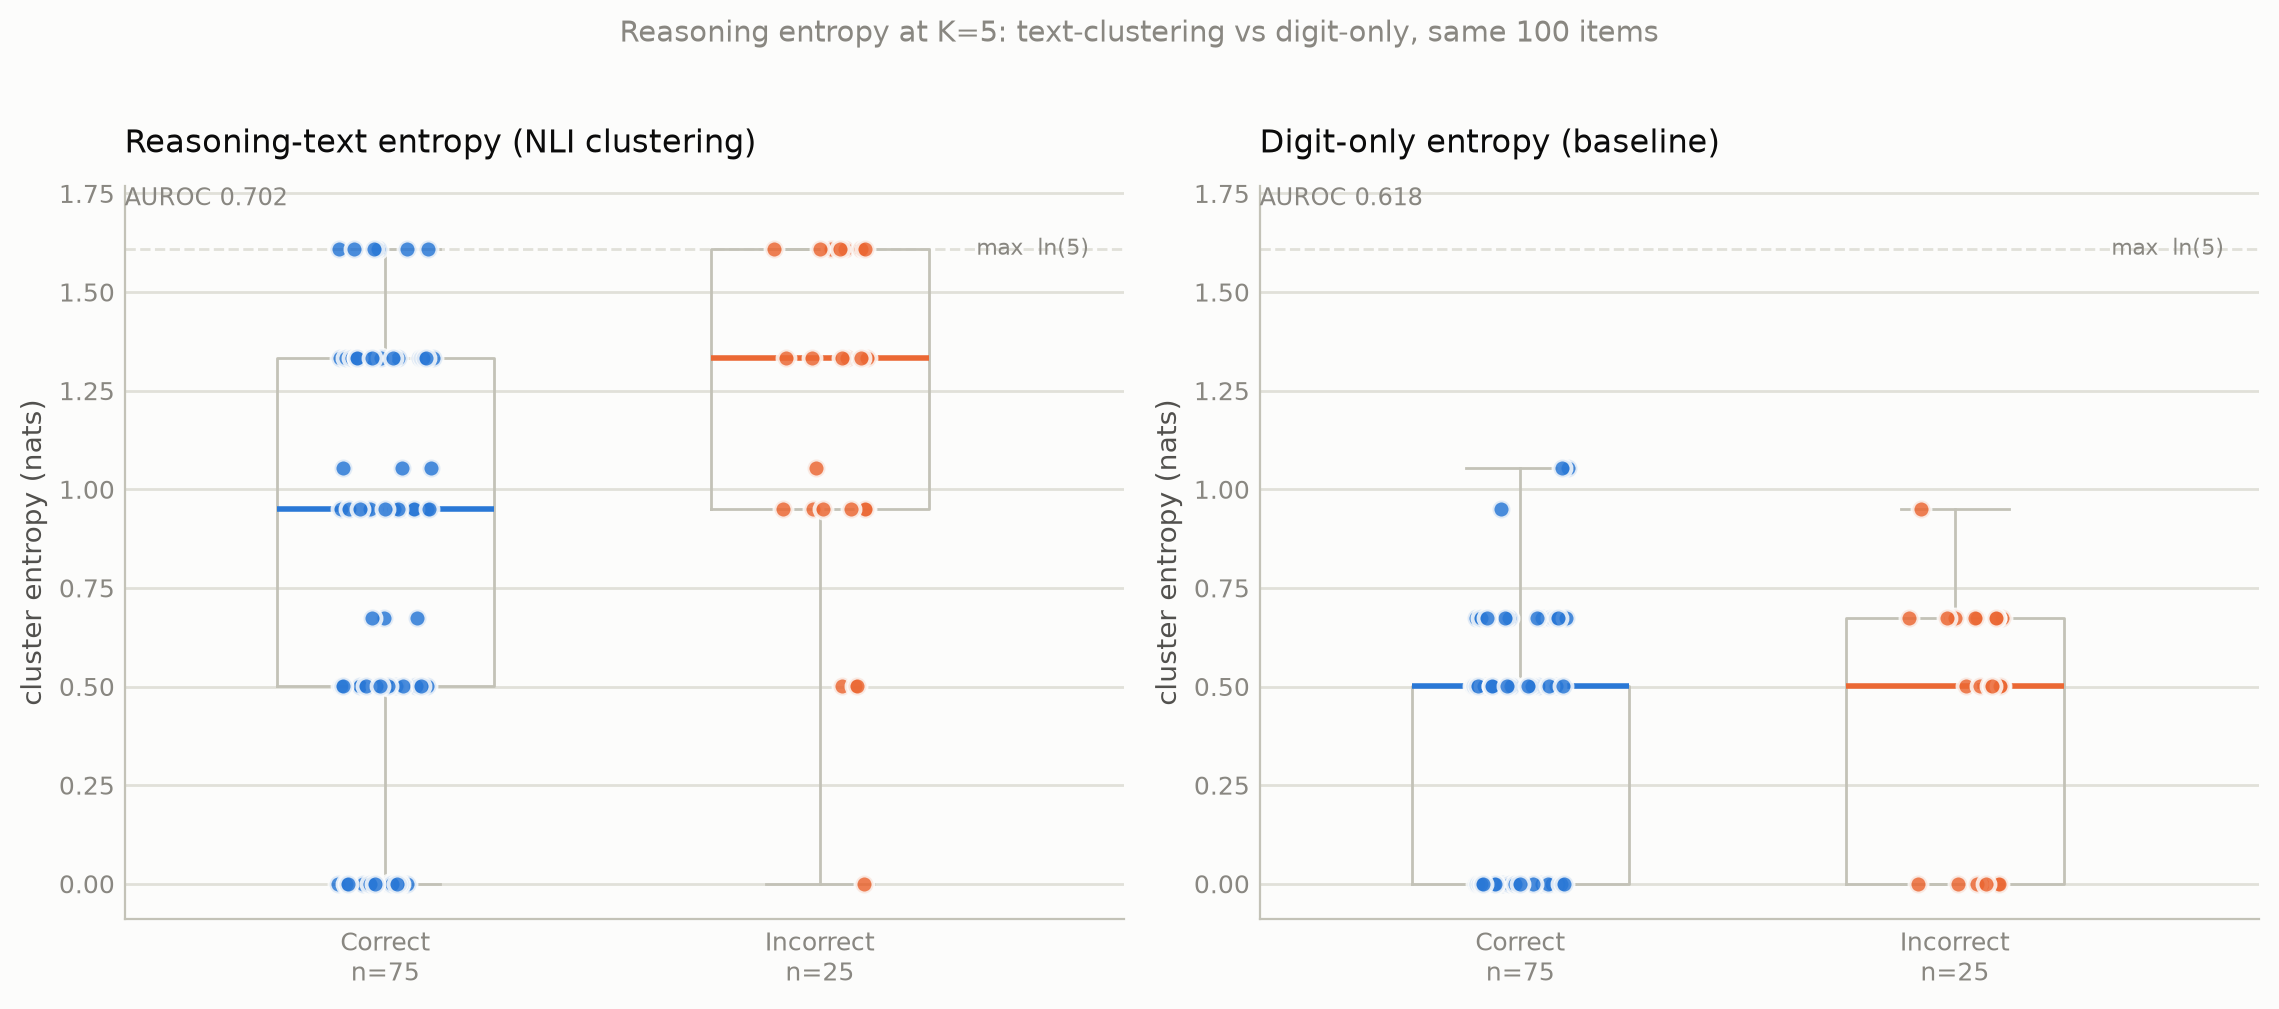
\includegraphics[width=\textwidth]{figures/reasoning_text_vs_digit_entropy.png}
  \caption{Reasoning entropy at $K=5$: clustering the model's reasoning text
  (left, AUROC 0.702) vs. the digit-only baseline (right, AUROC 0.618), same
  100 items. The reasoning-text approach separates the incorrect group's
  median well above the correct group's; the digit-only approach ties them
  exactly.}
  \label{fig:reasoning-text}
\end{figure}

\section{Limitations}

\begin{itemize}
  \item \textbf{Single model, single run size.} All results are Qwen2.5-VL-3B
    on 100 items; no comparison to a larger model (7B) or a baseline
    uncertainty method.
  \item \textbf{No statistical inference.} No confidence intervals, no
    significance testing (DeLong's test, bootstrap) -- explicitly out of
    scope for this pass.
  \item \textbf{Perception correctness label is strict.} Transcription
    correctness requires the extracted final answer to match ground truth
    after canonicalization; some ``incorrect'' classifications are plausibly
    extraction-span mismatches (the model's answer and the ground truth
    landing in different canonicalization tiers) rather than genuine
    disagreement, which would mean the true accuracy is somewhat higher than
    42\%. This biases the reported accuracy conservatively, not favorably.
  \item \textbf{No human double-grading.} Ground-truth labels are taken as
    given from the dataset.
  \item \textbf{Reasoning entropy's ceiling is model- and task-specific.} The
    binary-outcome information limit applies to \emph{this} grading task
    design; a differently-posed prompt (e.g. eliciting a confidence score
    rather than a forced binary decision) was not tested.
  \item \textbf{Reasoning-text clustering is validated at $K=5$ only.} The
    cross-digit merge check (55 cases, 8 manually inspected) supports that the
    AUROC~$=0.702$ result is not the same NLI over-merging bias found in
    perception Attempt~2, but this has not yet been confirmed at $K=15$, and
    the underlying cross-encoder is a small, general-purpose NLI model rather
    than one tuned for mathematical reasoning text.
\end{itemize}

\section{Recommended Next Steps}

\begin{enumerate}
  \item \textbf{Complete the $K=15$ GPU confirmation} of reasoning-text
    clustering (\texttt{pilot/02\_reasoning\_text\_entropy.ipynb}) and fold the
    result into this report. The $K=5$ result is validated but a second, larger
    $K$ strengthens confidence the same way it did for the digit-only signal.
  \item \textbf{Token-level confidence as an alternative reasoning signal.}
    Instead of inferring uncertainty from repeated discrete sampling, use the
    model's own next-token probability for the 0/1 decision at generation
    time. A richer, more direct signal, but requires new sampling code and a
    new run to validate.
  \item \textbf{Scale to a stronger model (7B) or the full dataset} only after
    deciding whether the reasoning arm's current best result (0.702) is
    acceptable as-is or worth the additional investment above.
\end{enumerate}

\end{document}
